\date{}
\documentclass[fleqn, a5paper]{amsart}
\usepackage[top = 2cm, bottom = 2cm, left = 2cm, right = 2cm, a5paper]{geometry}
\usepackage{amsmath, amssymb, amsthm}
\usepackage{marginnote}
\usepackage{gensymb}
\usepackage{commath}
\usepackage{xcolor}
\usepackage{cancel}
\usepackage{siunitx}
\usepackage{tikz, pgfplots}
	\usetikzlibrary{calc, hobby, patterns, intersections}
\usepackage{graphicx}
\usepackage{hyperref}
\usepackage{datetime}
\usepackage{ulem}
\usepackage{xfrac}
\usepackage{asymptote}
\usepackage{enumerate}
\usepackage{float}
\setcounter{secnumdepth}{4}
\newcommand\numberthis{\addtocounter{equation}{1}\tag{\theequation}}

\newcommand{\AxisRotator}[1][rotate=0]{%
	\tikz [x=0.25cm,y=0.60cm,line width=.2ex,-stealth,#1] \draw (0,0) arc (-150:150:1 and 1);%
}

\theoremstyle{definition}
\newtheorem{example}{Example}
\newtheorem{definition}{Definition}

\theoremstyle{theorem}
\newtheorem{theorem}{Theorem}

\newenvironment{solution}
{\begin{proof}[Solution]\let\qed\relax}
	{\end{proof}}

\newcommand{\curl}{\mathrm{curl\,}}

%\renewcommand{\int_{min}^{max}}{\int\displaylimits_{min}^{max}}

%opening
\title{Physics 1 : Compendium}
\author{Aakash Jog}

\begin{document}

\maketitle
%\setlength{\mathindent}{0pt}

\section{Non-Linear Motion}

\begin{align*}
	\overrightarrow{r} &= r \hat{r} \\
	\overrightarrow{v} = \dot{\overrightarrow{r}} &= \dot{r} \hat{r} + r \dot{\theta} \hat{\theta} \\
	\overrightarrow{a} = \ddot{\overrightarrow{r}} &= \left(\ddot{r} - r(\dot{\theta})^2\right) \hat{r} + \left(2 \dot{r} \dot{\theta} + r \ddot{\theta}\right) \hat{\theta}
\end{align*}

\section{Conservative Forces}
	\begin{align*}
		\curl \overrightarrow{F} &\doteq \overrightarrow{\nabla} \times \overrightarrow{F} \\
		&=
			\begin{vmatrix} 
				\hat{x} & \hat{y} & \hat{z} \\
				\dpd{}{x} & \dpd{}{y} & \dpd{}{z} \\
				F_x & F_y & F_z \\
			\end{vmatrix}
	\end{align*}
	If $\overrightarrow{F}$ is conservative, $\curl \overrightarrow{F} = 0$.
	\begin{equation*}
		F = - \dod{U}{r}
	\end{equation*}
\section{Conservation of Momenta}

\begin{example}
	On one side of a boat of mass $M$, a box of mass $m$ is placed and the boat's engine is pulling the box via a massless rope. At $t = 0$ the entire system is at rest. Then the engine is turned on and it starts pulling the box with force $\overrightarrow{F}(t) = \alpha t$ where $\alpha$ is a positive constant. The friction coefficients between the box and the boat are $\mu_s$ and $\mu_k$. The engine is working for time $\tau = \dfrac{mg}{\alpha}$ and then stops. Assuming that the box does not reach the end of the boat nor collide with any other object, what will be the boat's velocity after a very long time $t >> \tau$? Find the box's velocity w.r.t. the boat from the moment the engine is turned on.
\end{example}

\begin{solution}
	\begin{align*}
		F &= \alpha t &;\quad 0 \leq t \leq \tau = \dfrac{mg}{\alpha}\\
		N_s &= \mu_s m g\\
		N_k &= \mu_k m g
	\end{align*}
		Let $t_0$ be the time when the box starts moving.
	\begin{align*}
		F(t) &= \mu_s m g\\
		&= \alpha t\\
		\therefore t_0 &= \dfrac{\mu_s m g}{\alpha}
	\end{align*}
		For $t_0 < t < \tau$,
	\begin{align*}
		\alpha t - \mu_k m g &= m a\\
		\therefore a &= \dfrac{\alpha t}{m} - \mu_k g\\
		\therefore v &= \int\limits_{t_0}^{\tau} a(t) \dif t\\
		&= \dfrac{\alpha}{2m} (\tau^2 - t_0^2) - \mu_k g (\tau - t_0)
	\end{align*}
		For $t > \tau$,
	\begin{align*}
		a &= \mu_k g\\
		\therefore v &= v_{\tau} + \int\limits_{\tau}^{t} g \dif t\\
		&= v_{\tau} - \mu_k g (t - \tau)
	\end{align*}
\end{solution}

\section{Rigid Body Motion}

\subsection{Gyroscope}
A disk is attached to rods as shown, and is rotating about itself with $\omega$.\\
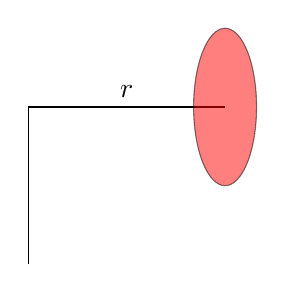
\begin{tikzpicture}[scale = 0.5]
	\def\y{4};
	\def\x{5};
	\def\R{2};
	
	\draw (0,0) -- (0,\y);
	\draw (0,\y) -- (\x,\y) node [midway, above] {$r$};
	
	\filldraw [fill = red, opacity = 0.5] (\x,\y) circle [x radius = 0.4*\R, y radius = \R];
\end{tikzpicture}\\
The torque is directed $\otimes$.\\
Seen from the top,\\
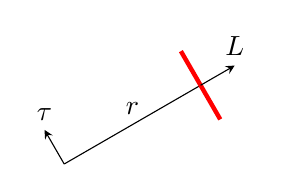
\begin{tikzpicture}[scale = 0.5]
	\def\r{4};
	\def\R{1};
	\def\angle{30};
	\def\F{1};

	\draw (0,0) -- (\angle:\r) node [midway, above] {$r$};
	\draw [ultra thick, red] (\angle:\r) -- ++({90 + \angle}:\R);
	\draw [ultra thick, red] (\angle:\r) -- ++({-90 + \angle}:\R);
	
	\draw [-stealth] (0,0) -- ++({90 + \angle}:\F) node [above] {$\tau$};
	\draw [-stealth] (\angle:\r) -- ++(\angle:\F) node [above] {$L$};
\end{tikzpicture}\\
\begin{align*}
	\overrightarrow{\tau} &= \tau \hat{\theta}
\end{align*}
with respect to the joint,
\begin{align*}
	\overrightarrow{L} &= \dfrac{1}{2} m R^2 \omega \hat{r}\\
	\therefore \dod{\overrightarrow{L}}{t} &= \dfrac{1}{2} m R^2 \omega \cdot \dod{\hat{r}}{t}\\
	\therefore \tau &= \dfrac{1}{2} m R^2 \omega \dot{\theta}\\
	\therefore m g r &= \dfrac{1}{2} m R^2 \omega \dot{\theta}
\end{align*}
Therefore,
\begin{align*}
	\dot{\theta} &= \dfrac{2 g r}{R^2 \omega}
\end{align*}

\begin{example}
	A disk of mass $m$ and radius $R$ is fixed on a rod and is kept on two stands fixed on another disk which is rotating with $\Omega$. Find the normal forces that the stands are exerting on the rod.\\
	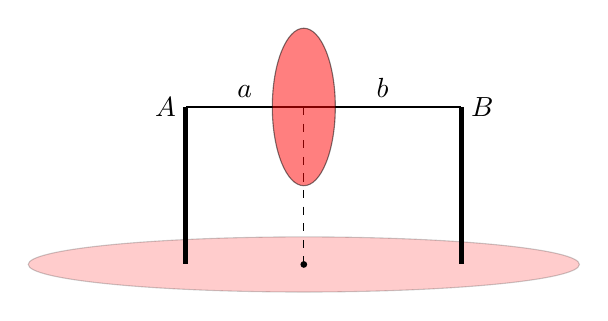
\begin{tikzpicture}[scale = 0.5]
		\def\z{4};
		\def\a{3};
		\def\b{4};
		\def\R{2};
		
		\coordinate (disk centre) at (0,\z);
		\coordinate (A) at (-\a,\z);
		\coordinate (B) at (\b,\z);
		
		\filldraw [fill = red, opacity = 0.2] (0,0) circle [x radius = {\a + \b}, y radius = {0.1*(\a + \b)}];
		
		\filldraw (0,0) circle [radius = 2pt];
		
		\draw [ultra thick] (A) -- ++(-90:\z);
		\draw [ultra thick] (B) -- ++(-90:\z);
		
		\node at (A) [left] {$A$};
		\node at (B) [right] {$B$};
		
		\draw (disk centre) -- (A) node [midway, above] {$a$};
		\draw (disk centre) -- (B) node [midway, above] {$b$};
		
		\draw [dashed] (disk centre) -- (0,0);
		
		\filldraw [fill = red, opacity = 0.5] (0,\z) circle [x radius = 0.4*\R, y radius = \R];
	\end{tikzpicture}\\
	\begin{tikzpicture}
	
	\end{tikzpicture}
\end{example}

\begin{solution}
	As viewed from the top,\\
	\begin{tikzpicture}[scale = 0.5]
		\def\angle{30};
		\def\a{4};
		\def\b{4};
		\def\F{3};
		
		\draw [-stealth, red] (0,0) -- (\angle:1) node [above] {$\hat{r}$};
		
		\draw [-stealth, red] (0,0) -- ({90 + \angle}:1) node [above right] {$\hat{\theta}$};
		
		\draw [dashed] (0,0) -- (\angle:\b) node [above right] {$N_B$};
		\node at (\angle:\b) {$\odot$};
		
		\draw [dashed] (0,0) -- ({180 + \angle}:\a) node [above left] {$N_A$};
		\node at ({180 + \angle}:\a) {$\odot$};
		
		\draw [-stealth] (0,0) -- (\angle:\F) node [above] {$L$};
		\draw [-stealth] (0,0) -- ({90 + \angle}:\F) node [above] {$\tau_A$};
		\draw [-stealth] (0,0) -- ({-90 + \angle}:\F) node [below] {$\tau_B$};
	\end{tikzpicture}\\
	About the point $O$,
	\begin{align*}
		\overrightarrow{L} &= \dfrac{1}{4} m R^2 \Omega \hat{z} + \dfrac{1}{2} m R^2 \omega \hat{r}\\
		\therefore \overrightarrow{\tau} &= \dod{\overrightarrow{L}}{t}\\
		&= \dod{}{t} \left( \dfrac{1}{4} m R^2 \Omega \hat{z} + \dfrac{1}{2} m R^2 \omega \hat{r} \right)\\
		&= \dod{}{t} \left( \dfrac{1}{2} m R^2 \omega \hat{r} \right)
	\end{align*}
	The net torque about point $O$ is only due to the normal forces.\\
	Therefore, the net torque is in the $\hat{\theta}$ direction. Hence, it cannot change the magnitude of $\omega$, but only the direction.\\
	Therefore,
	\begin{align*}
		\overrightarrow{\tau} &= \dod{}{t} \left( \dfrac{1}{4} m R^2 \Omega \hat{z} + \dfrac{1}{2} m R^2 \omega \hat{r} \right)\\
		&= \dfrac{1}{2} m R^2 \omega \dod{\hat{r}}{t}\\
		&= \dfrac{1}{2} m R^2 \omega \dot{\theta} \hat{\theta}\\
		&= \dfrac{1}{2} m R^2 \omega \Omega \hat{\theta}\\
		\therefore a N_A \hat{\theta} + b N_b (-\hat{\theta}) &= \dfrac{1}{2} m R^2 \omega \Omega \hat{\theta}
	\end{align*}
	Therefore,
	\begin{align*}
		a N_A - b N_B &= \dfrac{1}{2} m R^2 \omega \Omega
	\end{align*}
	Also,
	\begin{align*}
		N_A + N_B &= m g
	\end{align*}
\end{solution}

\section{Variable Mass Systems}

If a rocket is releasing gasses with velocity $u$ with respect to it,
\begin{equation*}
\dod{p}{t} = m \dod{v}{t} + \dod{m}{t} u
\end{equation*}

\section{Centres of Mass}

\begin{tabular}{l l}
	Solid hemisphere & $\left( \sfrac{3}{8} \right) R$\\
	Hollow hemisphere & $\left( \sfrac{1}{2} \right) R$\\
	Solid cone (from vertex) & $\left( \sfrac{3}{4} \right) h$\\
	Hollow cone (from vertex) & $\left( \sfrac{2}{3} \right) h$\\
\end{tabular}

\begin{example}
	Find the centre of mass of an eighth of a solid sphere.
\end{example}

\begin{solution}
	Consider an elemental mass $\dif m$ at $(r, \theta, \varphi)$.
	\begin{align*}
		x_{\text{COM}} &= \dfrac{\int\limits_{r = 0}^{R} \int\limits_{\theta = 0}^{\frac{\pi}{2}} \int\limits_{\varphi = 0}^{\frac{\pi}{2}} r \sin \theta \cos \varphi \dif V}{\iiint \dif V}\\
		&= \dfrac{\int\limits_{r = 0}^{R} \int\limits_{\theta = 0}^{\frac{\pi}{2}} \int\limits_{\varphi = 0}^{\frac{\pi}{2}} r \sin \theta \cos \varphi (r^2 \sin \theta \dif r \dif \theta \dif \varphi)}{\dfrac{1}{8} \cdot \dfrac{4}{3} \pi R^3}
	\end{align*}
	Therefore,
	\begin{equation*}
		\therefore x_{\text{COM}} = y_{\text{COM}} = z_{\text{COM}} = \dfrac{3}{8} R
	\end{equation*}
\end{solution}

\section{Moments of Inertia}

\begin{equation*}
	I = \int r^2 \dif m
\end{equation*}

\begin{tabular}{l l}
	Ring ($\perp$ to plane) & $m R^2$\\
	Disk ($\perp$ to plane) & $\left( \sfrac{1}{2} \right) m R^2$\\
	Solid sphere & $\left( \sfrac{2}{5} \right) m R^2$\\
	Hollow sphere & $\left( \sfrac{2}{3} \right) m R^2$\\
	Rod (centre) & $\left( \sfrac{1}{12} \right) m l^2$\\
	Rod (end) & $\left( \sfrac{1}{3} \right) m l^2$\\
	Cone (axis of symmetry) & $\left( \sfrac{3}{10} \right) m R^2$\\
\end{tabular}

\section{Accelerating Systems}

\begin{equation*}
	F_{\textnormal{centrifugal}} = - m \overrightarrow{\omega} \times \left( \overrightarrow{\omega} \times \overrightarrow{r} \right)
\end{equation*}
\begin{equation*}
	F_{\textnormal{coriolis}} = - 2 m \overrightarrow{\omega} \times \overrightarrow{v}
\end{equation*}

\section{Oscillations}

\subsection{Simple Oscillations}

\begin{equation*}
	\ddot{x} = - \omega^2 x
\end{equation*}

\begin{equation*}
	\omega_{\textnormal{physical pendulum}} = \sqrt{\dfrac{d_{\textnormal{axis,COM}} m g}{I_{\textnormal{axis}}}}
\end{equation*}

\subsection{Damped Oscillations}

\begin{equation*}
	\ddot{x} + \dfrac{\beta}{m} \dot{x} + {\omega_0}^2 x = 0
\end{equation*}

\begin{tabular}{c c}
	Strong damping & $\dfrac{\beta}{2m} > \omega_0$\\[2ex]
	Critical damping & $\dfrac{\beta}{2m} = \omega_0$\\[2ex]
	Weak damping & $\dfrac{\beta}{2m} < \omega_0$\\[2ex]
\end{tabular}\\
Oscillations occur in case of weak damping.\\

Let $\omega_1 = \sqrt{{\omega_0}^2 - \left( \dfrac{\beta}{2m} \right)^2}$.\\
For weak damping,
\begin{equation*}
	x = e^{-\sfrac{\beta}{2m} \cdot t} \left( \widetilde{A} \cos \omega_1 t + \widetilde{B} \sin \omega_1 t \right)
\end{equation*}
For critical damping,
\begin{equation*}
	x = e^{-\sfrac{\beta}{2m} \cdot t} \left( \widetilde{A} + \widetilde{B} t \right)
\end{equation*}
In case of strong damping,
\begin{equation*}
	x = \widetilde{A} e^{\left( -\sfrac{\beta}{2m} + \sqrt{-{\omega_1}^2} \right)} + \widetilde{B} e^{\left( -\sfrac{\beta}{2m} - \sqrt{-{\omega_1}^2} \right) t}
\end{equation*}

\subsection{Forced Oscillations}

\begin{align*}
	m \ddot{x} + \dfrac{k}{m} x &= \dfrac{F_0}{m} \cos \omega t\\
	\therefore \ddot{x} + \dfrac{k}{m} x &= \dfrac{F_0}{m} \cos \omega t
\end{align*}
Therefore, solving
\begin{align*}
	x &= A \cos \omega_0 t + B \sin \omega_0 t + \dfrac{F_0}{k - m \omega^2} \cos \omega t\\
	\therefore \dot{x} &= \omega_0 (-A \sin \omega_0 t + B \cos \omega_0 t) - \dfrac{F_0}{k - m \omega^2} \omega \sin \omega t
\end{align*}
Substituting initial conditions,
\begin{align*}
	x &= \dfrac{\dfrac{F_0}{m}}{\dfrac{k}{m} - \omega^2} (-\cos \omega_0 t + \cos \omega t)\\
	\intertext{Let $\dfrac{F_0}{m} = f_0$}
	\therefore x &= -\dfrac{2 f_0}{{\omega_0}^2 - \omega^2} \sin \left( \dfrac{\omega t - \omega_0 t}{2} \right) \sin \left( \dfrac{\omega t + \omega_0 t}{2} \right)\\
	\intertext{$\omega - \omega_0 = \Delta \omega$ and $\omega + \omega_0 \approx 2 \omega_0$}
	\therefore x &\approx \dfrac{2 f_0}{\Delta \omega \cdot 2 \omega_0} \sin \left( \dfrac{\Delta \omega}{2} t \right) \cdot \sin (\omega_0 t)
\end{align*}

\end{document}